\begin{frame} \frametitle{\vspace*{0.5cm}Background on contrast-enhanced ultrasound bioeffects}
  \begin{figure}
    \centering
    \begin{tikzpicture}
      \node[anchor=south west,inner sep=0] (image) at (0,0) {
        \includegraphics[height=0.25\textheight]{./figs/CEUS}
      };%
      \begin{scope}[x={(image.south east)},y={(image.north west)}]%
        \node[font=\tiny,right] at (0.01,0.03) {\scalebox{0.4}{\textcolor{white}{\cite{Wei2001}}}};%
      \end{scope}%  
    \end{tikzpicture}\hfill%
    \begin{tikzpicture}
      \node[anchor=south west,inner sep=0] (image) at (0,0) {
        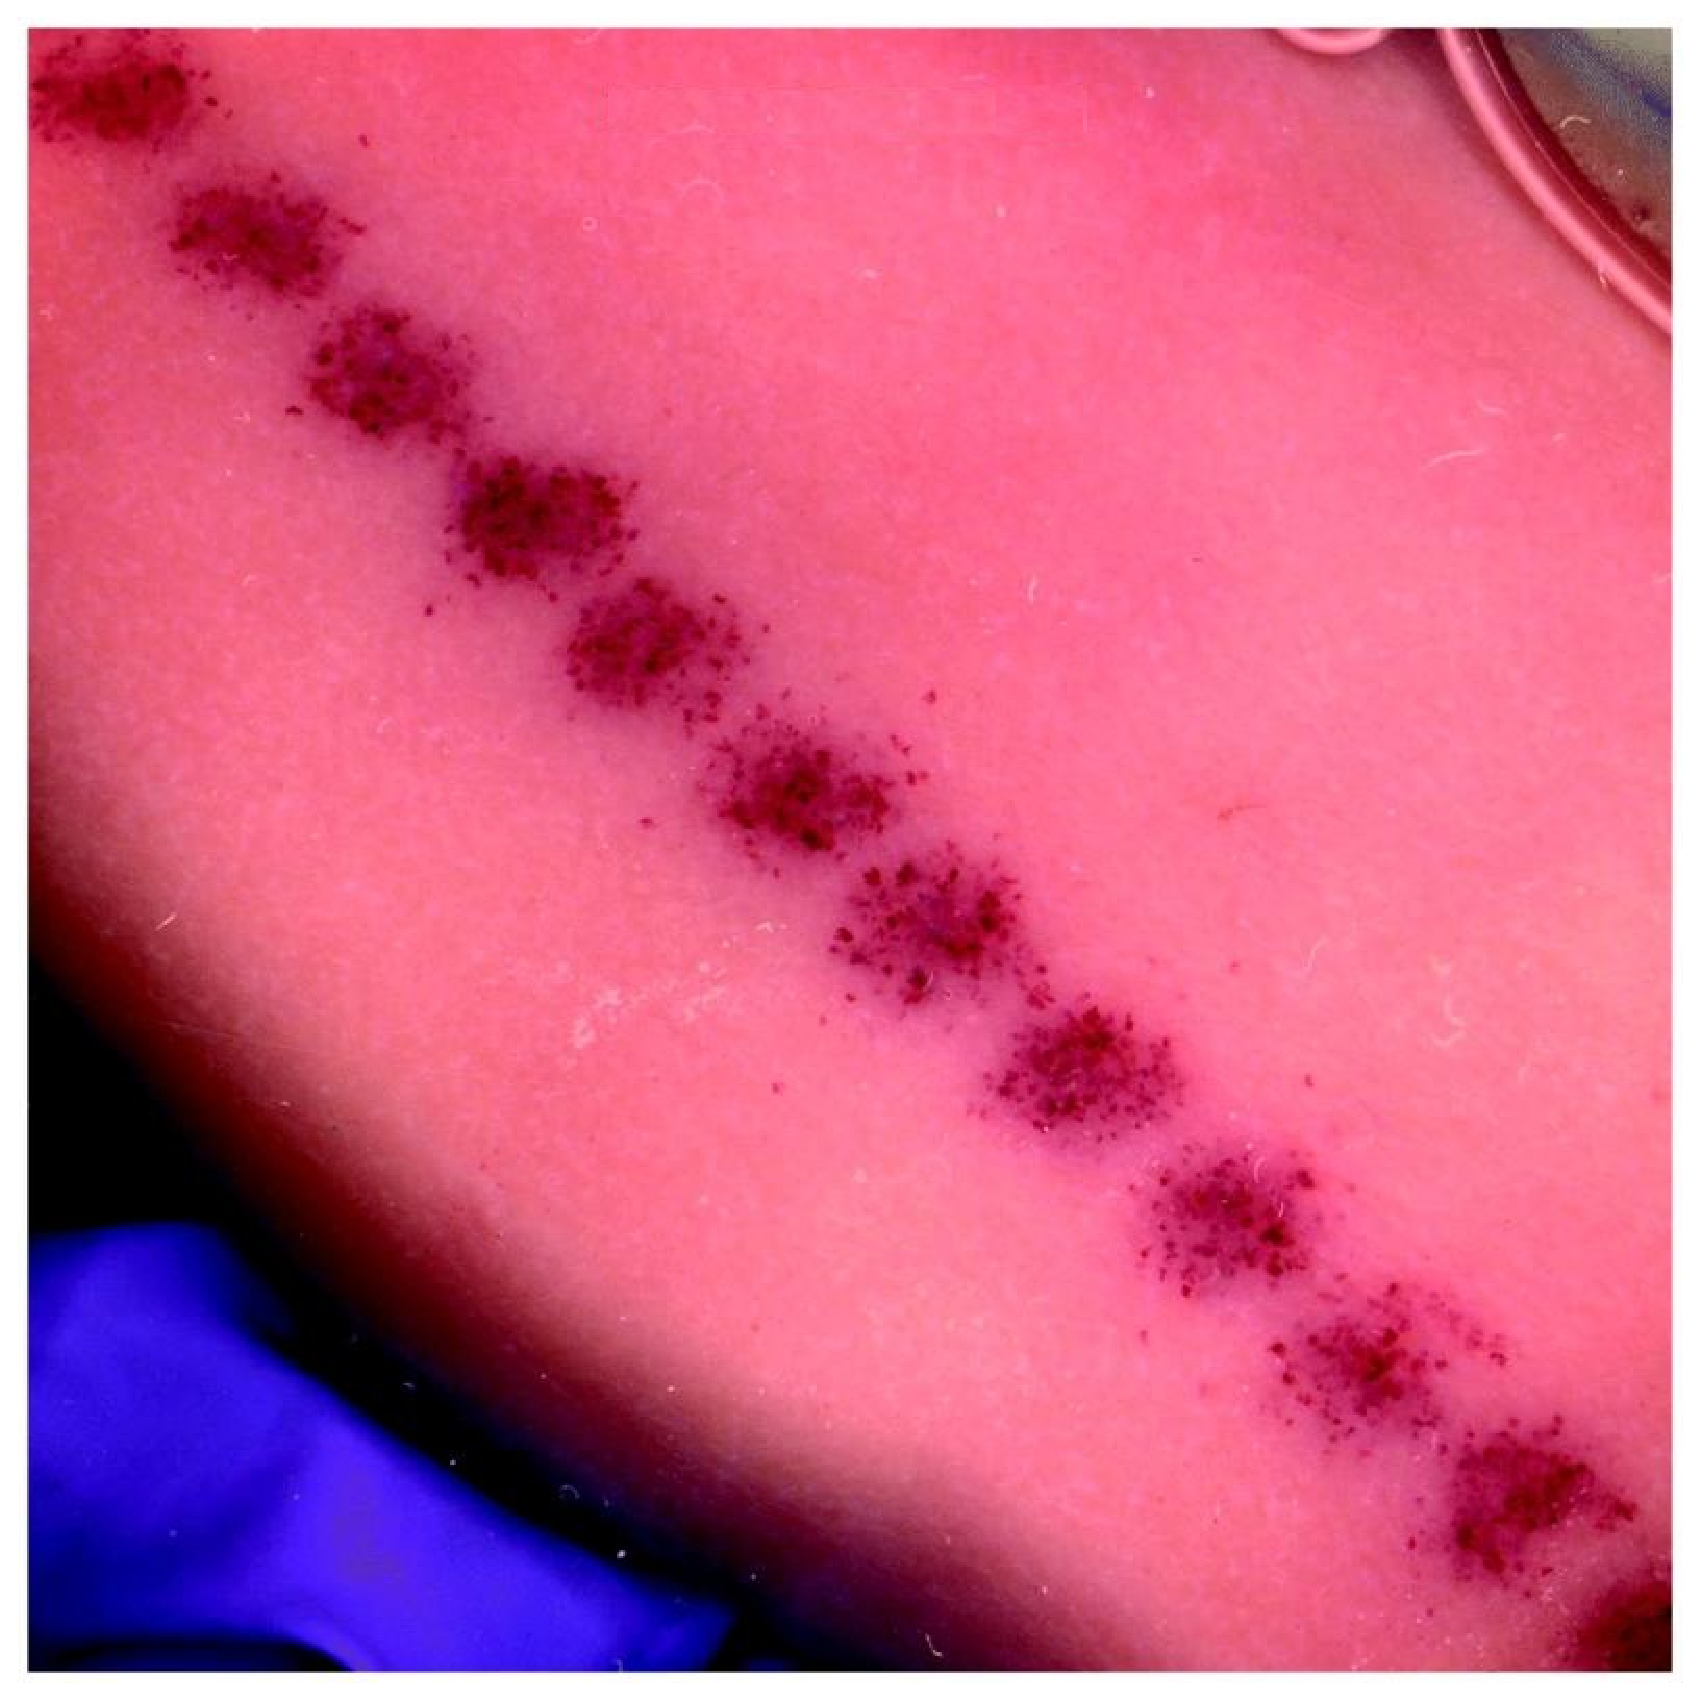
\includegraphics[height=0.25\textheight]{./figs/Kidney_Bleed}\hfill
      };%
      \begin{scope}[x={(image.south east)},y={(image.north west)}]%
        \node[font=\tiny,right] at (0.01,0.03) {\scalebox{0.4}{\textcolor{white}{Courtesy of D. L. Miller}}};%
      \end{scope}%  
    \end{tikzpicture}\hfill%
    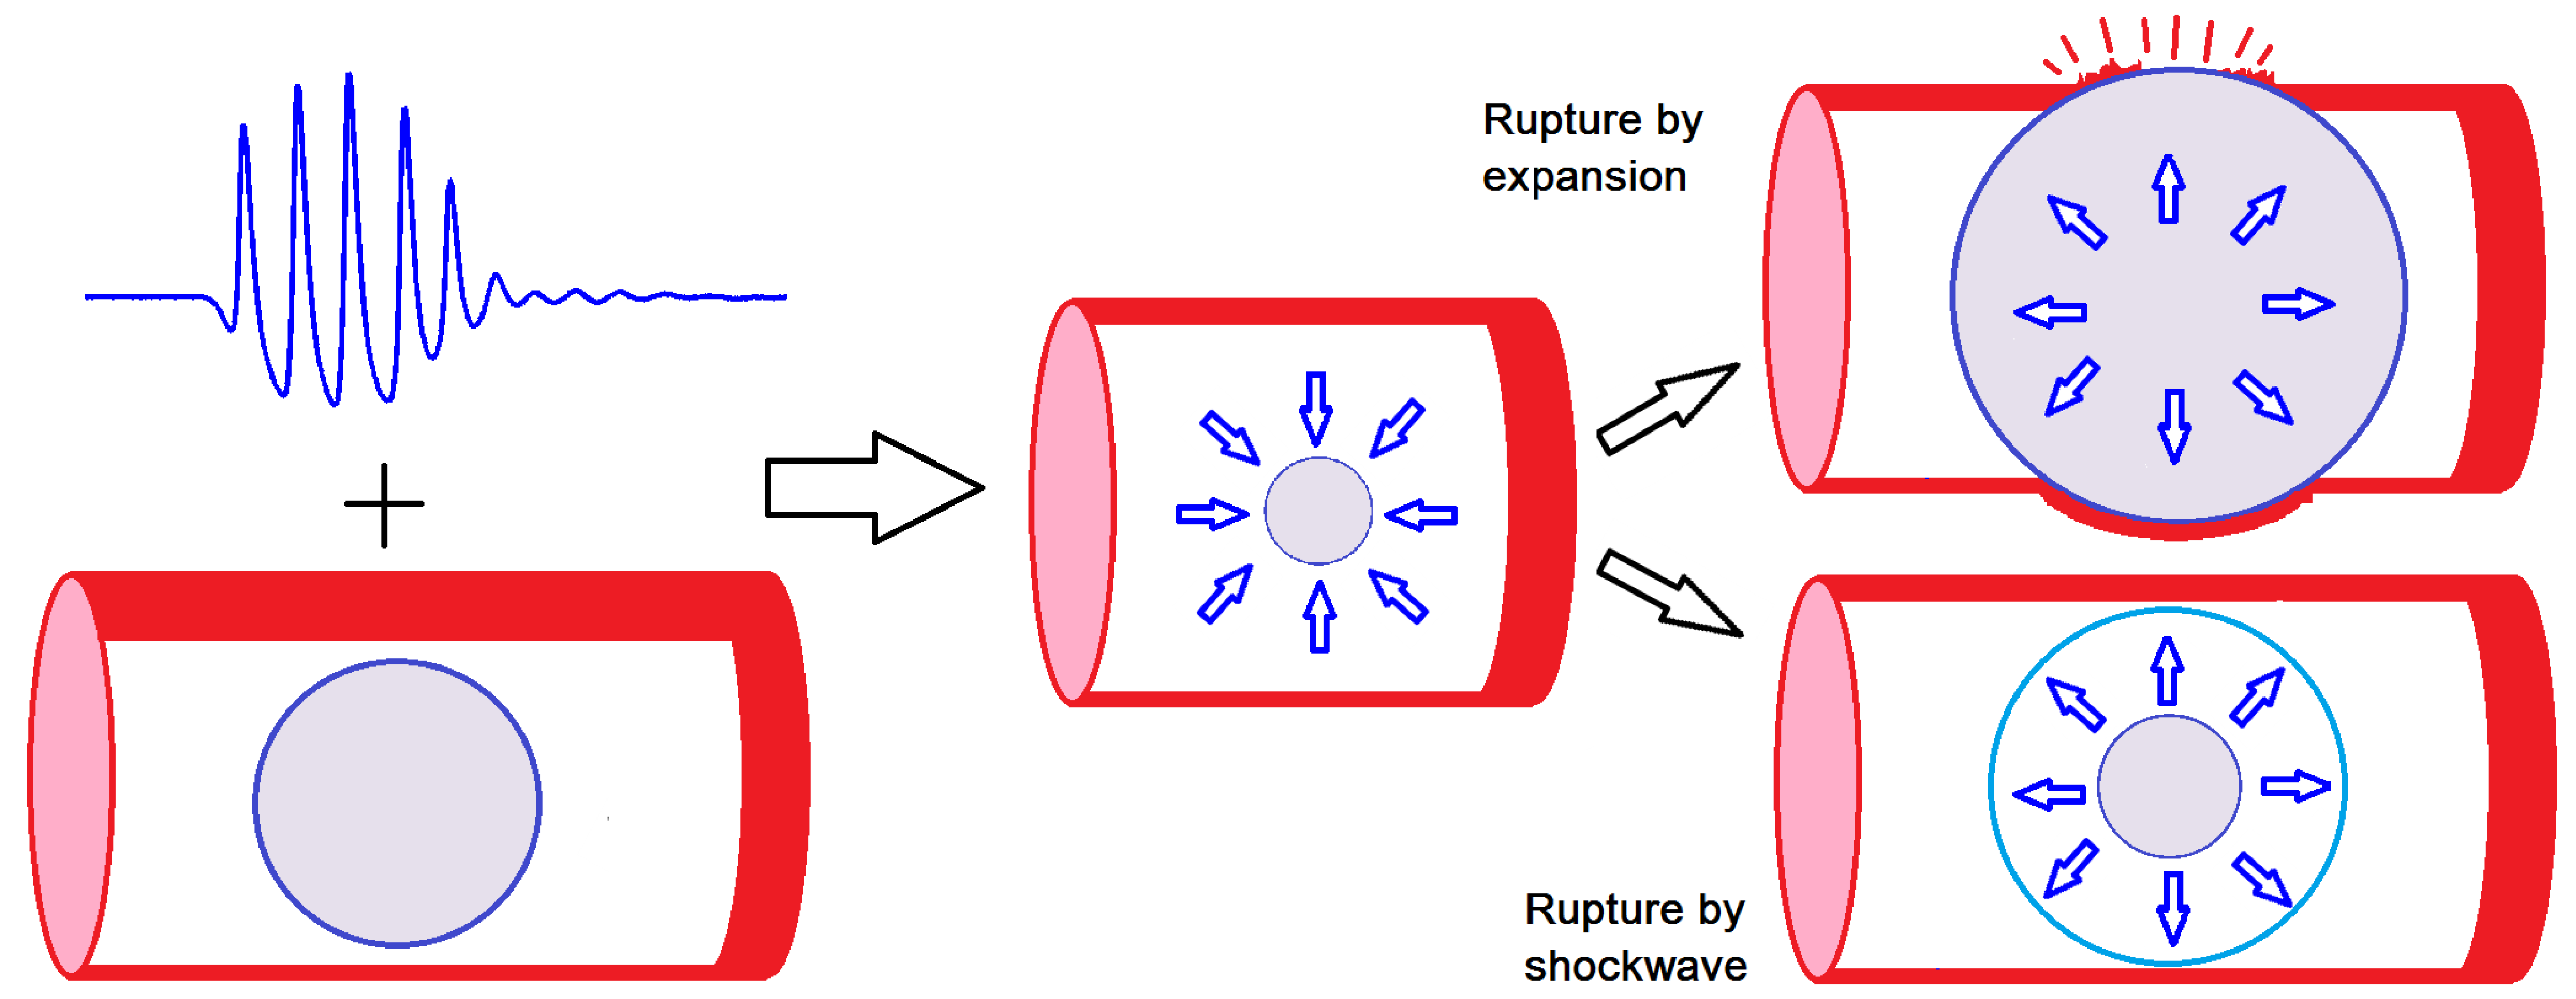
\includegraphics[height=0.25\textheight]{./figs/cavitation_hemorrhage}
  \end{figure}
  {\small
    \begin{itemize}
    \item Contrast-Ehanced Ultrasound (CEUS) provides high contrast diagnostic medical imaging in areas without high contrast (e.g., blood).
    \item CEUS uses echogenic microbubbles for contrast, and can lead to hemorrhage and cell death.
    \item Though cavitation of the microbubbles appears to be the
      cause, the exact mechanisms and thresholds are not well
      understood.
    \end{itemize}
  }
\end{frame}
%
%%% Local Variables:
%%% mode: latex
%%% TeX-master: t
%%% End:
